% This work is licensed under the Creative Commons
% Attribution-NonCommercial 3.0 Unported License. To view a copy of this
% license, visit http://creativecommons.org/licenses/by-nc/3.0/.

\section{Versuchsaufbau und Durchführung}

\subsection{Aufbau und Besonderheiten des Sagnac-Interferometers}
%
Das in diesem Versuch verwendete Sagnac Interferometer besteht im 
Kern aus einem Helium-Neon-Laser, welcher linear polarisiertes 
Licht mit einer Wellenlänge von \SI{632.8}{\nano\metre} liefert, 
fünf Spiegeln, einem PBSC und einem Polarisationsfilter.\\
Des Weiteren werden für spezielle Messverfahren noch ein weiterer 
PBSC, ein weiterer Polarisationsfilter und zwei Photodioden 
verwendet, sowie zur Untersuchung der Brechungsindices zwei im 
festen Winkel zueinander angeordnete Glasplatten und eine Gaskammer.\\
Eine schematische Zeichnung des Interferometers, sowie Skizzen der 
zusätzlichen Bauteile sind in Bild~\ref{fig:bauteile} zu sehen.\\
Der Einsatz der einzelnen Bauteile wird in den Untersektionen 
der jeweiligen Messverfahren erläutert.\\
Alle Bauteile werden an einem Schraubbrett befestigt und während 
der Messungen von einem Plexiglasdach überdacht, um Luftströmung 
innerhalb der Interferometeranordnung zu verhindern.\\
Die Besonderheit dieses Interferometertyps liegt in der 
Toleranz gegenüber Vibrationen der Apparatur, da die gegenläufigen 
Strahlen die selben Weglängen zurücklegen und somit die 
Phasendifferenz weitestgehend unverändert bleibt. Außerdem können  
bei diesem Interferometetyp, so wie für Interferometer üblich, die 
einzelnen Strahlen seperat manipuliert werden, da diese einen 
räumlichen Abstand zueinander besitzen.\\
%
\begin{figure}[]
  \centering
  \includegraphics[width=1\textwidth]{figures/bauteile}
  \caption{Schematische Skizze der verwendeten Apparatur, sowie der 
   Glasplattengeometrie und der Gaskammer. Der durchgezogene Strahl 
    repräsentiert den Lichtweg, wenn die beiden gegenläufigen 
    Strahlen nicht räumlich getrennt sind, die gestrichelten Linien 
     deuten den Weg der räumlich getrennten Lichtstrahlen an.
    Diese Skizze wurde mit 
    dem Programm Inkscape selber erstellt.}
  \label{fig:bauteile}
\end{figure}
%
\subsection{Justierung der Apparatur}
%
Die Justierung des Sagnac Interferometers wird mittels der in 
Zeichnung~\ref{fig:bauteile} verwendeten Bezeichnung der Spiegel 
und Halteplätze für Justierhilfen erläutert. Die Justierhilfen 
sind Plastikplatten mit kleinen Löchern zum durchlassen des 
Laserlichts.\\
Als erstes werden der HeNe-Laser und die beiden 
Steuerspiegel auf dem 
Schraubbrett befestigt. Außerdem werden der PBSC und 
die Spiegel A, B und C wie in~\ref{fig:bauteile} zu sehen platziert, 
aber noch nicht festgeschraubt.
 Diese werden nun in ihre endgültige Position gebracht.
Dafür wird zunächst der durch den PBSC reflektierte Teilstrahl 
blockiert und Justierhilfen in den Halterungen Zwei und Drei 
angebracht. Mit dem zweiten Steuerspiegel wird der durch den PBSC 
durchgelassene Teilstrahl so eingestellt, dass dieser die Löcher 
beider Justierhilfen passiert.\\
Als nächstes werden die Justierhilfen in die Halterungen Acht und 
Neun gestellt, der vom PBSC durchgelassene Teilstrahl blockiert und 
der reflektierte Teilstrahl durch Feinjustage des PBSCs so 
eingestellt, dass dieser nun ebenfalls die Justierhilfen passiert. 
Nun wird der PBSC festgeschraubt.\\
Nachdem dies erledigt ist, werdne die Justierhilfen in die Plätze 
Fünf und Sechs gesteckt, keiner der Teilstrahlen blockiert und 
Spiegel A und C so lange zurechtgerückt, bis die Lichtstrahlen 
einmal mehr durch Löcher der Justierhilfen gelangen. Jetz 
werden Spiegel A und C festgeschraubt.\\
Ein letztes mal werden die Justierhilfen umverlegt. Diesmal 
in die Halterungen Vier und Sieben. Spiegel C wird zurechtgerückt, 
bis beide Teilstrahlen durch jeweils beide Seiten der Löcher der 
Justierhilfen gelangen. Spiegel C wird daraufhin auch an dem 
Schraubbrett festgeschraubt.\\
Zu diesem Zeitpunkt sind die beiden Teilstrahlen im Interferometer 
noch nicht räumlich getrennt. Werden die aus der vierten Seite des 
PBSCs austretenden Lichtstrahlen auf einem Schirm betrachtet, zeigt 
sich aber, dass die beiden Lichtstrahlen sich nicht vollkommen 
überlappen. Um dies zu erreichen, werden die Fingerschrauben bei 
den Spiegeln A und C verwendet. Nach diesem Schritt sind die Spiegel 
richtig justiert.\\
Vor dem PBSC wird noch ein Polarisationsfilter gestellt, um die 
Intensitäten der beiden Teilstrahlen im Interferometer einstellen 
zu können, sowie der zweite Steuerspiegel seitlich bewegt, um 
eine räumliche Trennung der beiden Strahlen zu erreichen.\\
Jetzt ist die Hauptanordnung des Sagnac Interferometers justiert. 
Vor jeder Messreihe wird allerdings ein wenig an den Fingerschrauben 
der Spiegel A, B und C gedreht, um die Qualität der austretenden 
Strahlen zu optimieren.
Die beiden austretenden Strahlen sind zueinander senkrecht 
polarisiert, interferieren also noch nicht miteinander.\\
%
\subsection{Messung des Kontrasts}
%
Zur Kontrastmessung wird zusätzlich zum justierten Interferometer 
ein zweiter Polfilter hinter dem PBSC, bei den austretenden Strahlen, 
aufgestellt, damit bei beiden Strahlen nur den Teil durchlassen, 
welcher im richtigen Winkel steht und diese durchgelassenen 
Komponenten interferieren können. Des Weiteren wird eine 
Photodiode verwendet, deren Photostrom in eine dazu proportionale 
Spannung umgewandelt wird, welche mit einem Voltmeter gemessen wird, und 
die in Abbildung~\ref{fig:bauteile} gezeigte Glasplattengeometrie 
benutzt. Diese wird so in das Innere des Interferometers gestellt, 
dass je einer der Glasplatten in einem der gegenläufigen Teilstrahlen 
steht.

Die Messreihe zur Bestimmung des Kontrastes des Interferometers 
in Abhängigkeit vom eingestellten Winkel des ersten 
Polarisationsfilters wird wie folgt durchgeführt:
Bei festem Polarisationsfilterwinkel wird die Glasplattengeometrie 
so gedreht, dass die am Voltmeter angezeigt Spannung minimal wird. 
Anschließend wird bei gleich bleibender Plattenposition die 
angezeigte Spannung in Abhängigkeit des Polarisationsfilterwinkels 
aufgezeichnet.

Im Anschluss dazu wird die Glasplattengeometrie so gedreht, dass 
die angezeigte Spannung maximal wird und eine weitere 
Messreihe bei fester Plattenposition gestartet, bei der für 
verschiedene Polarisationswinkel die Spannung abgelesen wird.
An dieser Stelle sei bereits darauf hingewiesen, dass dieses Vorgehen 
sich als nicht ideal erweist.
%
\subsection{Messung des Brechungsindex' von Glas}
%
Um die Brechzahl von Glas zu bestimmen, werden neben dem 
justierten Sagnac Interferometer noch die Glasplattengeometrie, 
ein zweiter, schräg stehender PBSC mit Spiegeln zum Interferieren und 
räumlichen Trennen der aus dem Interferometer kommenden Teilstrahlen, 
sowie zwei Photodioden benutzt. Mit dem Photostrom der 
Photodioden wird wieder jeweils eine dazu proportionale 
Spannung erzeugt. Diese Spannungen werden voneinander subtrahiert. 
Da die Intensitäten der aus dem zweiten 
PBSC kommenden Strahlen zueinander komplementär sind, ergibt die 
Betrachtung der Spannungsdifferenz eine Methode zum Feststellen von 
$2\pi$-Phasenshifts zwischen den beiden Interferometerstrahlen anhand 
von Spannungsdifferenznulldurchgängen. Diese Phasenshifts werden 
elektronisch gezählt.

Die Messung wird durchgeführt, indem die Glasplattengeometrie um 
\SI{10}{\degree} um die vertikale Achse gedreht wird und die Anzahl 
der $2\pi$-Phasenshifts abgelesen wird. Daraufhin werden die 
Glasplatten wieder um \SI{10}{\degree} zurückgedreht und die neue 
Anzahl an Phasenshifts notiert. Dieser Vorgang wird zehn mal 
wiederholt.
%
\subsection{Bestimmung der Brechungsindices von Luft und Kohlendioxid}
%
Im letzten Messteil, der Bestimmung der Brechzahl von Luft oder 
anderen Gasen, wird neben den Bauteilen im Teil zur Bestimmung 
der Brechzahl von Glas noch eine Gaskammer verwendet, welche 
an einer Vakuumpumpe angeschlossen ist. Die Gaskammer wird so 
in das Interferometer gestellt, dass nur einer der gegenläufigen 
Interferometerstrahlen das Gasmedium durchquert.\\
Vor der Messung wird die Gaskammer evakuiert. Das Einlassen von 
Gas führt zu einer Erhöhung der Dichte des in der Kammer befindlichen 
Mediums, wodurch sich ebenfalls die Brechzahl des Gases ändert und es 
zu einer Phasenverschiebung zwischen den Strahlen kommt.
In einer Messreihe wird die Anzahl der gezählten 
$2\pi$-Phasenverschiebungen in Abhängigkeit vom Druck in der 
Gaskammer gezählt.\\
Es werden sowohl Luft, als auch C02 vermessen.
%
